	\section{Condiciones óptimas}
	Esta parte de la aplicación permite llevar a cabo la optimización de costes.
	
	
	Para calcular la conversión óptimas se usa la siguiente expresión:
	
	\begin{equation*}
		X_{A_{opt}} = 1- \frac{C_Ra}{(\Delta w) C_{A0}VK}
	\end{equation*}
	
	Para calcular el tiempo óptimo se usa la siguiente expresión:
	
	\begin{equation*}
		t_{opt} = \frac{1}{K}\ln \left(\frac{(\Delta w) C_{A0}VK}{C_Ra}\right)
	\end{equation*}
	
	Los parámetros necesarios para el cálculo de las condiciones óptimas son:
	
	\begin{itemize}
		\item Orden de reacción.
		\item Temperatura inicial [K].
		\item Concentración inicial [mol/l].
		\item Energía de activación [J/mol].
		\item Constante $k_0$.
		\item Volumen [m3].
		\item Coste de reacción [€/s]
		\item Valor aumentado por mol transformado [€].
	\end{itemize}
	
	En la Figura \ref{con_op} se puede ver la ventana para el cálculo de las condiciones
	óptimas para la reacción.

	\begin{figure}[!h]
		\centering
		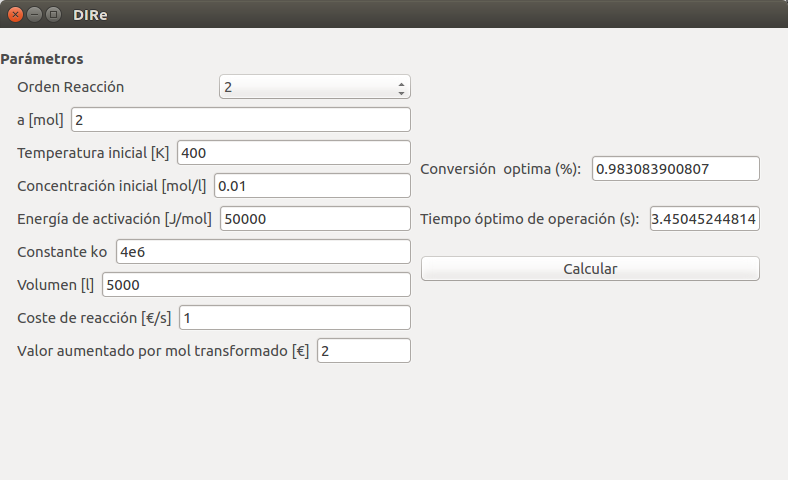
\includegraphics[width=0.9\textwidth]{./imagenes/reactor_discontinuo/con_op.png}
		\label{con_op}
		\caption{Ventana para el cálculo de las condiciones óptimas para la reacción.}
	\end{figure}

	